\documentclass[a4paper]{article}
\usepackage{geometry}
% Set the margins
\geometry{
    a4paper,
    total={170mm,257mm},
    left=20mm
}

\usepackage{csvsimple}
\usepackage{subcaption}
\usepackage{listings}
\usepackage{xcolor}

\definecolor{codegreen}{rgb}{0,0.6,0}
\definecolor{codegray}{rgb}{0.5,0.5,0.5}
\definecolor{codepurple}{rgb}{0.58,0,0.82}
\definecolor{backcolour}{rgb}{0.95,0.95,0.92}

\lstdefinestyle{mystyle}{
    backgroundcolor=\color{backcolour},   
    commentstyle=\color{codegreen},
    keywordstyle=\color{magenta},
    numberstyle=\tiny\color{codegray},
    stringstyle=\color{codepurple},
    basicstyle=\ttfamily\footnotesize,
    breakatwhitespace=false,         
    breaklines=true,                 
    captionpos=b,                    
    keepspaces=true,                 
    numbers=left,                    
    numbersep=5pt,                  
    showspaces=false,                
    showstringspaces=false,
    showtabs=false,                  
    tabsize=2
}
\lstset{style=mystyle}
\usepackage{subcaption}
\usepackage{graphicx}
\graphicspath{{./Images/}}

\title{COMP24112 Lab Report}
\author{Licheng Chen}

\begin{document}
\maketitle

\section{Linear Classification via Gradient Descent}

\subsection{Derivation of the training objection function}

$$O = C \sum^N_{i=1}\max\left(0, 1 - y_i \left(\mathbf{w}^T\mathbf{x}_i + w_0\right)\right) + \frac{1}{2}\mathbf{w}^T\mathbf{w}. $$


\newpage
\subsection{Model Training and Testing}
\begin{figure}[htbp]
    \centering
    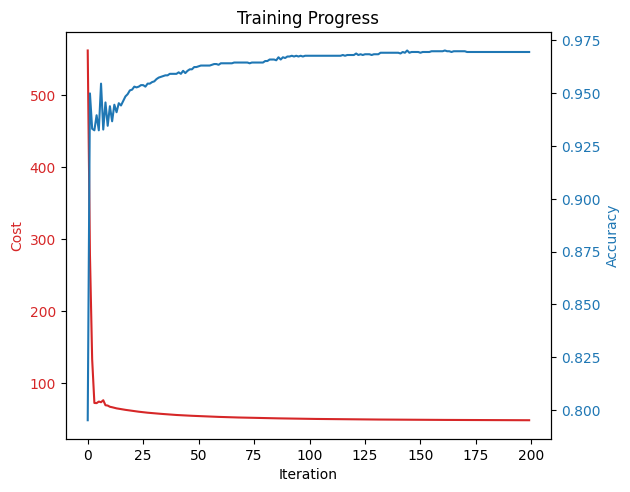
\includegraphics[width=0.5\linewidth]{1.11.png}
    \caption{\centering Graph of the cost and accuracy of training over iterations}
\end{figure}

The model produced by the run shown above had an accuracy of 0.9657 and an F1 score of 0.7213 when run on the test data. While initially very high, the cost of each iteration reduced dramatically, quickly falling below 100 before stabilising after ~10 iterations. In the first 25 iterations, the accuracy was rather spiky, suggesting that the model's parameters are oscillating around the optimal values before stabilising in the later iterations. This is probably caused by the fact that I chose to initialise my weights as zeros instead of randomising them, as this behaviour was not observed when I used randomised weights.

\subsection{Learning Rate Analysis}

\begin{figure}[htbp]
    \centering
    \begin{subfigure}[b]{0.49\linewidth}
        \centering
        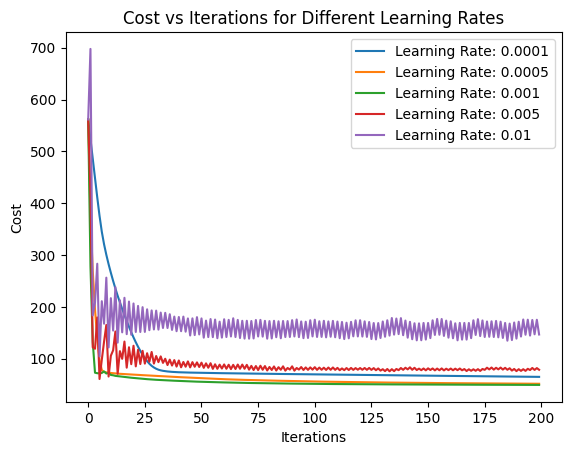
\includegraphics[width=\linewidth]{1.21.png}
        \caption{\centering Costs per iteration for various learning rates.}
    \end{subfigure}
    \hfill
    \begin{subfigure}[b]{0.49\linewidth}
        \centering
        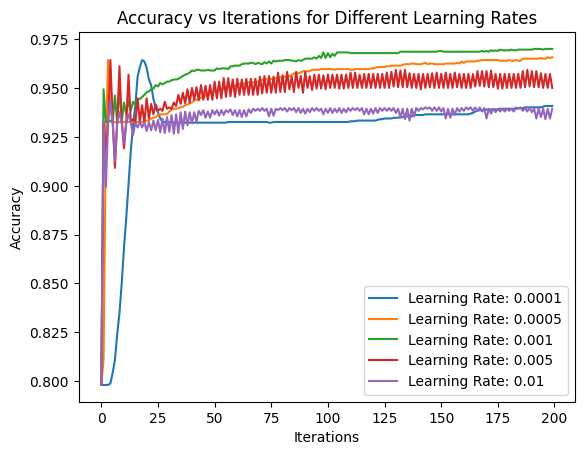
\includegraphics[width=\linewidth]{1.22.png}
        \caption{\centering Accuracy per iteration for various learning rates.}
    \end{subfigure}
    \caption{\centering Comparison of costs and accuracy per iteration for various learning rates.}
\end{figure}

The above graphs suggest that the most optimal learning rate seems to be 0.001. That value had the highest consistent accuracy when training, while 0.0001 initially had a higher accuracy, it dropped down to below that of 0.001 before it stabilised. The rates above 0.001 never stabilised at all. The costs are also higher the larger the learning rate is, except for 0.0001, which is higher than both 0.0005 and 0.001.

\newpage
\begin{figure}[htbp]
    \centering
    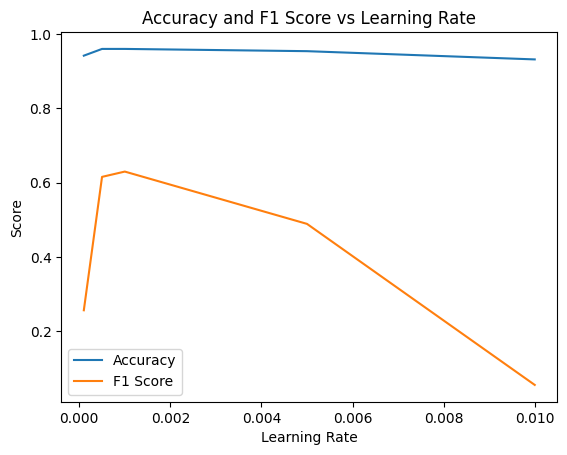
\includegraphics[width=0.5\linewidth]{1.23.png}
    \caption{\centering Graph of the accuracy and F1 score of of various learning rates.}
\end{figure}

The accuracy peaked at 0.0005, however the difference between that and 0.001 is marginal, while the F1 score peaked at 0.001, dropping sharply on both sides.

\newpage
\section{Air Quality Analysis by Neural Network}
\subsection{Model Selection}

The results reported that ReLU is the best activation function and the best hidden layer size is (100,100) with a cross-validation MSE of 0.1609.
The standard deviation of cross-validation MSE is 0.1617, which suggests some variability in model performance across different folds of the cross-validation.
The MSE on the test set is 0.2064, which is slightly higher than the cross-validation MSE. However, an \( R^2 \) score of 0.9071 suggests that the model explains approximately 90.71\% of the variance in the CO(GT) values on the test set. This indicates that the model generalizes well to unseen data.

\subsection{Training Algorithm Comparison: SGD and ADAM}
\begin{figure}[htbp]
    \centering
    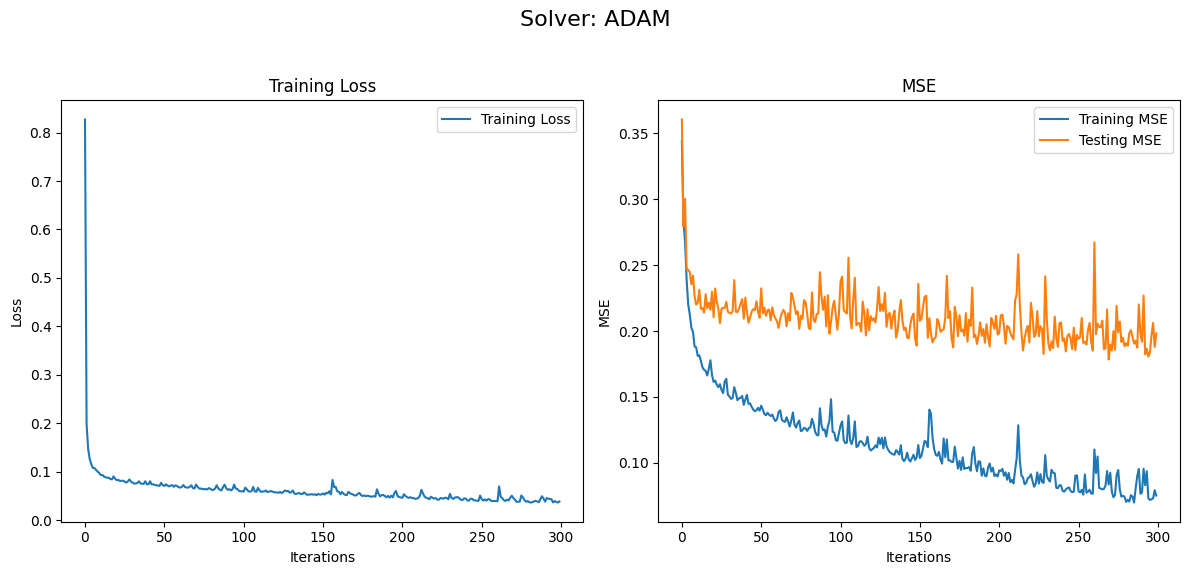
\includegraphics[width=0.9\linewidth]{2.11.png}
    \caption{\centering Loss and MSE of ADAM}
\end{figure}

\begin{figure}[htbp]
    \centering
    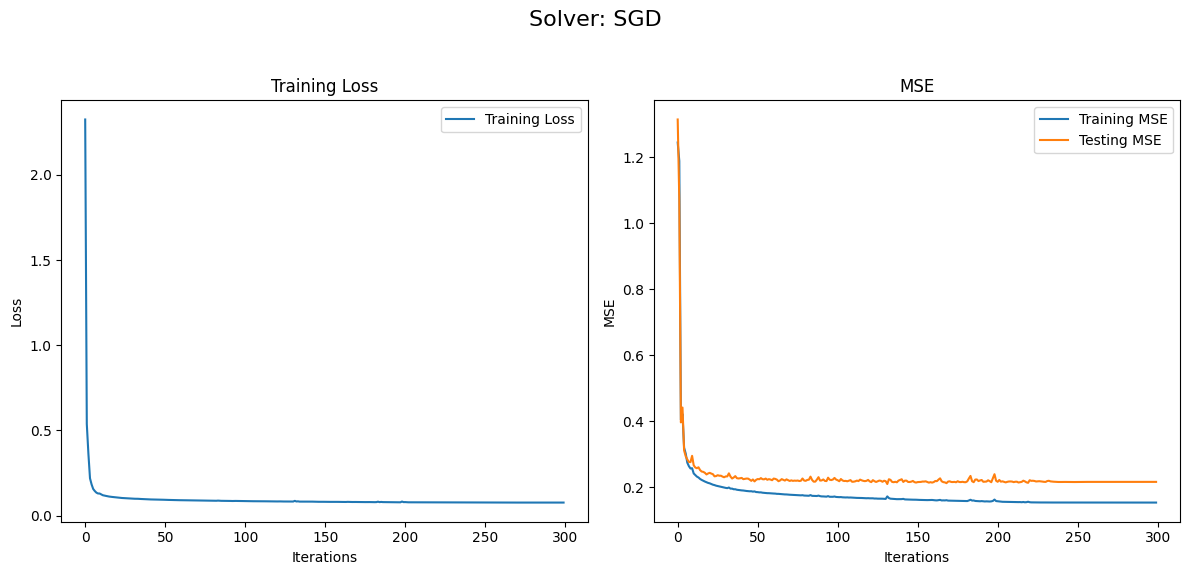
\includegraphics[width=0.9\linewidth]{2.12.png}
    \caption{\centering Loss and MSE of SGD}
\end{figure}
With a test MSE of 0.1983 and an \( R^2 \) score of 0.9108, ADAM appears to perform better than SGD. For SGD, the test MSE and \( R^2 \) score are 0.2157 and 0.9029, respectively, both of which are worse than those obtained with ADAM. However, the difference in performance seems marginal, as the gap between the two algorithms is only around 0.02 for MSE and 0.01 for the \( R^2 \) score.



\newpage
\section{Building A Robust MLP Regressor}


\end{document}